\subsection{Utilization vs Performance per Watt}
In traditional CPU-based datacenters, the optimum operating range is set and managed around 50-60\% core utilization across the datacenter. This is because the CPU processing elements are designed to operate for an average case load at peak energy efficiency~\cite{wong2016peak} in terms of performance per watt (PPW). Figure~\ref{fig:efficiency} plots the PPW of Memcached queries served by CPUs and GPUs, at different query load scenarios, where PPW is normalized with the PPW at 100\% load. For the CPU-bound queries, we observe that the peak energy efficiency at around 60\% to 70\% core utilization, but the PPW drops when utilization is further pushed by overclocking. We can see that the GPUs are fundamentally different from CPUs as their peak performance per watt is achieved only at 100\% load utilization of Streaming Multiprocessors (SMs). In case of Memcached-GPU~\cite{memcachedgpu} running individual queries are not energy proportional unless multiple queries are batched together. Batching multiple small queries is critical for energy efficiency while intuitively maximizing the throughput. However, operating the GPU at its peak energy efficiency and performance depends on the system scheduler's resource management policies.

\textbf{Design point 1:} \textit{Keeping the GPU utilization high is essential for high performance per watt.} 

\subsection{Cluster Workload Analysis}
In order to obtain very high utilization in GPUs, we need to know the application behavior in terms of resource request and usage trend. First, we focus on CPU specific workloads and later correlate the application behavior to GPU specific workloads. We analyze the recently open-sourced Alibaba production datacenter traces~\cite{baba} to gain insights into the nature of batch and latency critical jobs that are submitted to the CPU based datacenter and their corresponding resource consumption trends. Further, we investigate the inter-arrival times between these jobs to establish expected load at any given time for a production datacenter.

Alibaba's cluster traces were collected across 1300 CPU-based machines for a period of 12 hours at a granularity of every 60 seconds. We analyze both the batch and container workload behavior of 12,951 batch and 11,089 online service queries (containerized workload) in terms of their corresponding resource consumption trends. We summarize the following key observations: 

%There is a significant relationship between the cores, system load and memory resource consumption of latency-sensitive service jobs. Especially the system load recorded over the time are tightly correlated.
\begin{itemize}[wide, nosep, labelindent = 0pt, topsep = 0.3ex]
\item \textbf{Resource overcommitment - } Firstly, users tend to overstate their resource requirements. As observed from Figure~\ref{fig:cont-mem}, average CPU and memory utilization is 47\% and 76\% respectively. Half of the containers consume less than 45\% of the provisioned memory on an average. This over-consumption trend is also seen in CPUs, in which almost all the containers consume less than 50\% of the provisioned CPU cores. This is because, over-commitment indirectly helps to ensure the QoS of such queries by provisioning for the worst (peak) case. A cluster-wide resource orchestrator, while provisioning for an application, should not use the user-stated expected resource consumption as it leads to overall underutilization of the cluster. In case of CPUs, preemption and fine-grain resource sharing mitigates the problem, while it becomes a critical design point factor for a GPU scheduler. 

\textbf{Design Point 2:}\textit{ Due to varying resource needs of an application, instead of provisioning the resources for application's maximum utilization case, it is more resource efficient to provision for the average utilization case. It is ideal if the scheduler could dynamically provision and resize the containers based on the run-time growth of the application instead of static provisioning scheme.}\\

\item \textbf{Resource usage metrics are tightly correlated -}
Figure~\ref{fig:container} plots the Spearman's correlation across eight container resource utilization metrics as a heat map. Equation ~\ref{eqn:corr} gives the correlation score $\rho$ where, d$_{i}$ is the difference between the ranks (ordered in descending i.e, highest value gets rank 1 and lowest value gets rank 8) of corresponding utilization metrics in the heatmap and \textit{n} is the number of observations. Positive relationship between two metrics is represented by a score close to +1 and vice-versa. A score of 0.0 denotes that these metrics do not have any relationship. More positive the relationship, hotter is the color scheme (red). There is a significant relationship between the cores (core\_util), average system load recorded every second (load\_1) and memory resource consumption (mem\_util) of latency-sensitive service jobs. 
\end{itemize}
 \vspace{-1mm}
\begin{equation} 
\rho = 1-{}\frac{6 \Sigma d^{2}_i}{n(n^{2}-1)}
% r_{xy} = \frac{\sum x_i y_i - \sum x_i \sum y_i} {\sqrt{N \sum x_i^2 - (\sum x_i)^2} \sqrt{N \sum y_i^2 - \sum(y_i)^2}} 
\label{eqn:corr}
\vspace{-1mm}
\end{equation}

Figure~\ref{fig:batch} plots the correlation between six utilization metrics of batch workloads. It is seen that the memory utilization strongly correlates with the core utilization. Unlike latency sensitive queries, the batch applications exhibit strong correlation (both +vs \& -ve) between its utilization metrics. For example, the system load recorded over different sampling intervals, i.e. the Linux load average of the service instance usage at 1$^{st}$, 5$^{th}$and 15$^{th}$ second intervals, positively correlate with core utilization. On a similar note, CPU-utilization has a positive relationship with memory, but a negative relationship with the last level cache misses per kilo instructions (MPKI). This is a common trend across the workload.

This pair-wise correlation plot provides insights about latency sensitive application's resource usage behavior and the corresponding intertwined relationships across different resource usage metrics. It can be seen that the scheduler provisions for the dominant resource consumption (i.e., type of resource that is highly utilized)~\cite{Ghodsi:2011:DRF:1972457.1972490}. In case of co-located applications, the dominant resource type should not be the same. For example, co-locating a CPU bound application with a similar application would lead to severe SLA violations. 

\textbf{Design Point 3:}\textit{ Correlation between different resource utilization metrics need to be considered during placement to guarantee the performance of the scheduled application.}


% The production system scheduling policies are designed and optimized for CPUs and overlook accelerators like GPUs. We identify several GPU-based datacenter design choice issues and challenges below. 

 

\begin{figure}
\centering
  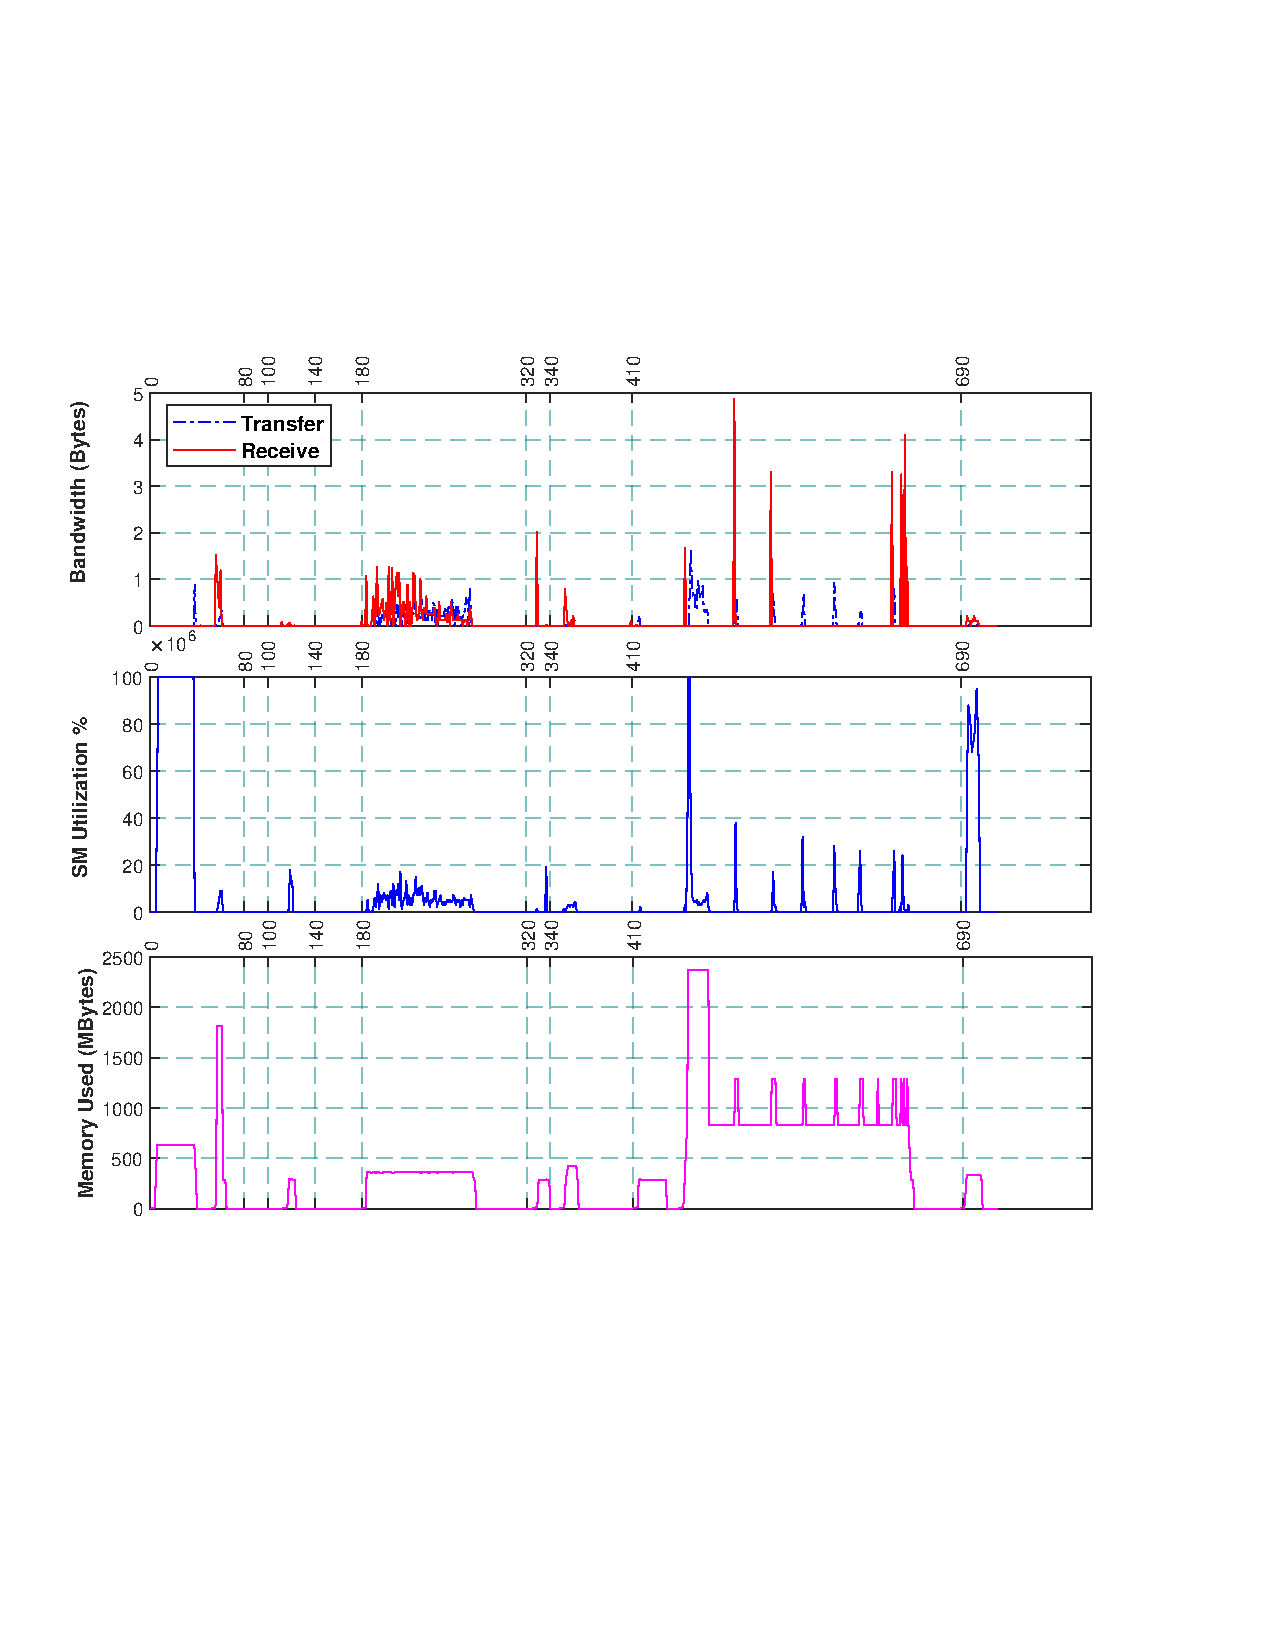
\includegraphics[width=0.99\linewidth ]
  {results/util.pdf}
  \vspace{-2mm}
  \caption{GPU Resource consumption of entire Rodinia suite on Nvidia's P100 GPU. The grid-lines mark the individual benchmark's runtime.(where x-axis is time in milliseconds)}
  \label{fig:rodinia-peaks}
\end{figure}



\subsection{GPU Workload Characterization}
We analyzed the resource consumption trends of both latency sensitive and batch workloads in Alibaba's production datacenter, which have correlating utilization metrics with respect to CPU, memory, disk, load, etc. Further, we apply this resource consumption trend to extend it to represent a GPU-based datacenter load and job inter-arrival scenario. To this end, we identified popular production workloads which subscribe to GPUs. Recall that GPU-based cloud services are becoming ubiquitous with the advent of Machine Learning as a Service (MLaaS)~\cite{gujarati2017swayam}. There have been significant industry-wide efforts on accelerating these queries through compute-intensive libraries such as cuDNN~\cite{ChetlurWVCTCS14}. These libraries are similar to MPI collective operations like broadcast, scatter-gather, all reduce, etc., and are specifically optimized for GPU data flow. 

The workloads use high-level libraries like Tensorflow, which are hosted as micro-service deployments as containers and are shipped via container orchestrators like Kubernetes~\cite{kubernetes}, Mesosphere~\cite{mesosp}, Docker swarm~\cite{swarm}, etc. Generally, these deployments are hosted as services such as object detection, feature extraction, etc. Queries to these containers arrive in short bursts, and the containers are also short-lived. For example, the average image recognition DNN-based inference query takes 90\textit{ms} on Nvidia P100 \cite{nvidia-dnn} whereas other batch jobs may run on a GPU for hours like an HPC application or even Proof-of-Work (PoW) for block-chain based crypto-currency mining.
%\subsection{Memory Fragmentation in Application Frameworks}
In order to create a representative workload mix for GPUs, which consists of both batch workloads and user-facing queries: (i) we use applications from Rodinia workload suite \cite{che2009rodinia} to mimic typical GPU bound HPC and compute-intensive workload submitted to the datacenters and, (ii) we use a mix of DNN based inference queries from Djinn and Tonic workload suite for user facing queries. \cite{hauswald2015djinn}. We execute each application from the workload on single GPU node to understand the batch-workload's resource demands. The details of the node are described in Table \ref{tbl:hw-config}. More details about the workload are explained further in Section \ref{sec:modeling}.

% \textbf{Design point 4:}\textit{ Ensuring the Quality of Service in case of applications that have stricter deadlines is an onus on the job scheduler.} 

\subsubsection{GPU Batch Workload}
Figure~\ref{fig:rodinia-peaks} plots different GPU resource consumptions over time for the eight different applications, which were run sequentially. We characterize memory used, Streaming Multiprocessor (SM) utilization and PCIe bandwidth which are three dominant resources for a batch application. It is observed that most of the applications could be co-located with one another since the resource consumption is relatively low. From Figure \ref{fig:rodinia-peaks}, we observe that the resource consumption of applications may not always peak at the same time. This temporal nature of the application resource usage can be exploited to avoid resource capacity violations, while sharing the resource. Further, we observe that these applications show a very deterministic pattern of phase changes. For example, typically if an application's input bandwidth activity is high, it is implied that the compute and memory would follow the same trend in near future. These subtle utilization cues could be picked up through real-time feedback and can be applied while making scheduling decisions. 

\textbf{Design point 4:} \textit{Batch application's utilization footprint is fairly predictable across the application's lifetime.}
% \vspace{-0.2in}
\subsubsection{GPU User-Facing Queries}
\label{sec:TF-mem-sec}
The Djinn and Tonic workload uses Tensorflow as its DNN application framework. TensorFlow(TF) not only provides the framework for executing ML queries but, also manages the execution flow of the query that run inside GPU. By default, TF earmarks the entire GPU memory despite actual workload demands. The TF runtime is designed to make this a default choice because GPUs are assumed to run a single context and not designed for multi tenant/application scenarios. In public datacenters to keep the operating costs low, it is ideal to share the GPUs because the individual application/tenant utilization is generally low. 

Figure~\ref{fig:tf-frag} shows the maximum memory consumption of different machine learning inferences. For most of the single inference queries, the memory consumption is less than 10\%. We batched these queries up to 128 queries per batch request, however, the majority of the inferences even with batching consume less than 50\% of the device memory. Whereas if the same application with the TF  application framework, they always earmark 99\% of the GPU memory causing severe internal memory fragmentation. This is a common case of resource overstatement from the workload behavior that we observed across Alibaba traces as explained in section \ref{sec:motivation}. 
% We do not consider SM utilization and PCIe bandwidth as they are not correlating as explained in Figure ~\ref{fig:container}. 
% When these inferences run inside TF-managed GPU, by default, the entire device memory is statically allocated for these inferences despite the actual consumption. 

Application frameworks like TF would always GPU resources by default leading to internal memory fragmentation. This directly affects the scheduler's global policies for fairness and performance. It is ideal for a datacenter scheduler to have two essential properties, namely, sharing incentive and strategy proofness~\cite{Ghodsi:2011:DRF:1972457.1972490}. In this case, neither can be ensured because the cluster-level resource manager has no control over the GPU device. In order to pack more applications to increase the utilization, the applications have to be provisioned by the datacenter scheduler by knowing the real-time GPU utilization metrics. 

\textbf{Design point 5:} \textit{It is essential to expose the application framework APIs to the job scheduler to avoid internal resource fragmentation.}

\begin{figure}
  \centering
  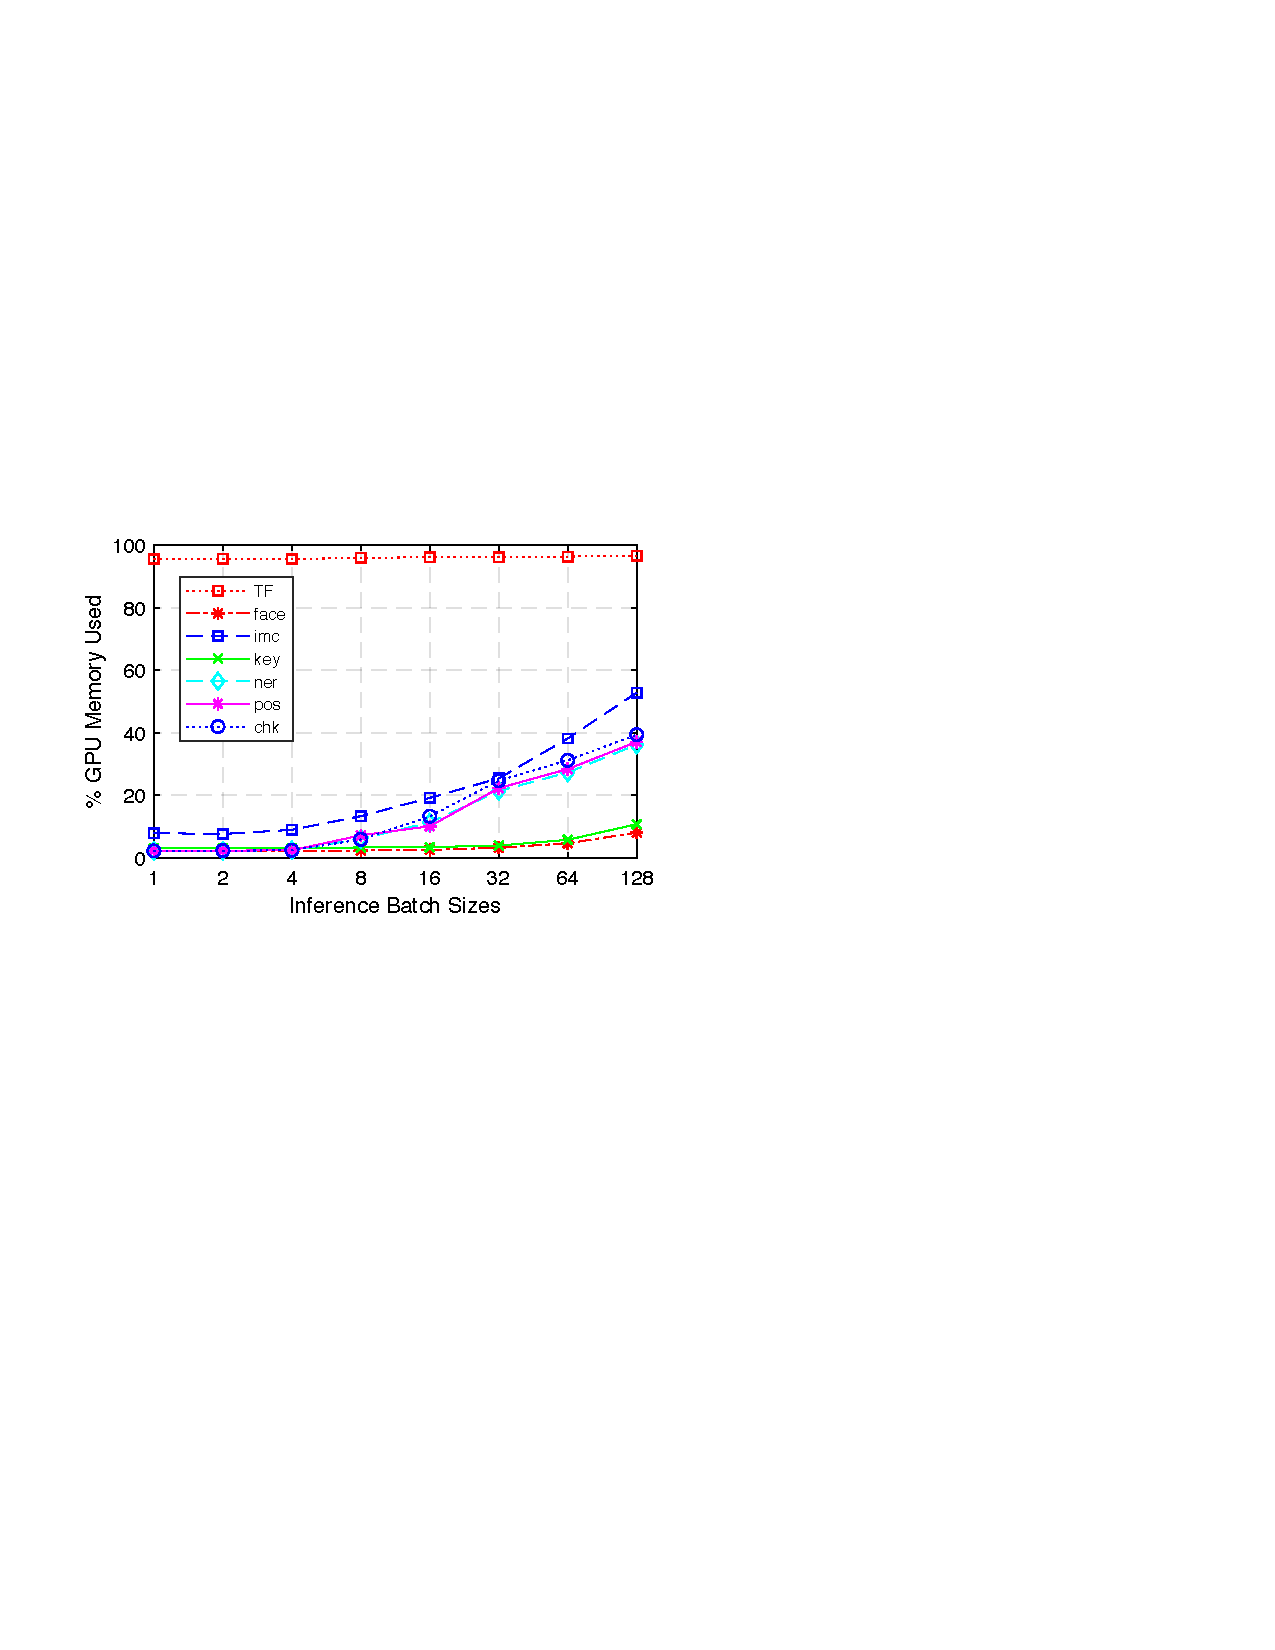
\includegraphics[width=.9\linewidth]{results/mem-fragmentation.pdf}
  \vspace{-2mm}
  \caption{Internal memory fragmentation of DNN inferences of Djinn and Tonic workload suite. TF is the Tensorflow managed memory consumption}
  \label{fig:tf-frag}
\end{figure}

% \item \textbf{Conservative scheduling policies -} 
% This results in a heavy imbalance of resource consumption trends, and it leads to resource fragmentation and poor energy efficiencies.
% \end{itemize}

% CPU systems are fairly resilient to these policies and overcome these challenges by resource virtualization, preemption, and load balancing. However, GPUs lack such support; therefore, CPU based resource orchestration and scheduling techniques cannot be applied to accelerators.


%%%%%%%%%Commented for space%%%%%%%%%%%%%%%%%%%%%%


% \vspace{-0.1in}
% \subsection{GPU Orchestration Challenges}
% Next, we explore the potential problems which will be encountered when both batch and user-facing queries are scheduled to the GPU concurrently. Although there are industry-wide efforts to support preemption of GPU kernels, still the technique is primitive and lacking when compared to CPUs. For example, when a batch task is scheduled on a GPU, the latency sensitive queries scheduled to the same node incur severe queuing delays and these kernels cannot be prioritized or run until the batch task finishes. By default, the uniform scheduler of Kubernetes is designed based on the fact that the GPUs are not shared across multiple containers. Therefore, ensuring QoS is entirely dependent on container startup latencies and queuing delays. The former could be mitigated by scheduling to a node which already has the container image. However, queuing delay is determined by both the kernels (apps) that currently are using the resources and the ones that are already ahead in the queue. Length of the queue can be a static indicator but however, just that would not suffice to guarantee the application turnaround time. Hence, real-time resource utilization feedback is an important metric for a scheduler to make effective orchestration decisions. Further, we do not make any changes to the application framework scheduler (tensorflow DAG scheduler) rather we augment \textit{Knots}, a GPU aware orchestration layer, to Kubernetes and design three scheduling schemes which leverage \textit{Knots}. 



%We discuss the challenges and how they are addressed in Section \ref{sec:modeling}. 

%\textbf{Design Point 6:}\textit{ GPU resource utilization metrics are critical to ensure the QoS of a particular application especially when they are co-located. An effective GPU resource scheduler would need to be dynamic and utilization aware.}

% To this end, as shown in Figure~\ref{fig:kubeknots}, we integrate {Knots}, an accelerator-aware orchestration layer with \textit{Kubernetes} which overcomes the above-listed challenges and enables cluster-wide GPU scheduling with end-to-end performance guarantees.
